%
\section{Experiments}
\label{sec:experiments}
%
% We evaluate \ourmethod{} on a broad range of time series forecasting and classification tasks. In Sec.~\ref{sec:empirical_realdata}, we test if \ourmethod{}'s contributions lead to state-of-the-art results on standard benchmarks. To help explain \ourmethod{}'s performance, in Sec.~\ref{sec:empirical_claims} we test if \ourmethod{}'s contributions actually improve their target criteria in practice. 
% We find that \ourmethod{} consistently obtains state-of-the-art results on popular time series benchmarks, and that these gains coincide with empirical improvements in expressiveness (Sec.~\ref{sec:empirical_expressivity}), forecasting flexibility (Sec.~\ref{sec:empirical_horizons}), and training efficiency (Sec.~\ref{sec:empirical_efficiency}). 

We test \ourmethod{} on a broad range of time series forecasting and classification tasks. In Sec.~\ref{sec:empirical_realdata}, we evaluate whether \ourmethod{}'s contributions lead to state-of-the-art results on standard benchmarks. To help explain \ourmethod{}'s performance and validate our contributions, in Sec.~\ref{sec:empirical_claims} we then evaluate whether these gains coincide with empirical improvements in expressiveness (Sec.~\ref{sec:empirical_expressivity}), forecasting flexibility (Sec.~\ref{sec:empirical_horizons}), and training efficiency (Sec.~\ref{sec:empirical_efficiency}). 

\subsection{Main Results: Time Series Forecasting and Classification}
\label{sec:empirical_realdata}
For forecasting, we evaluate \ourmethod{} on 40 forecasting tasks from the popular Informer~\citep{zhou2021informer} and Monash~\citep{godahewa2021monash} benchmarks, testing on horizons 8 to 960 time-steps long. For classification, we evaluate \ourmethod{} on seven medical ECG 
or speech audio classification tasks, which test on sequences up to 16,000 time-steps long. For all results, we report mean evaluation metrics over three seeds. \xmark~denotes the method was computationally infeasible on allocated GPUs, \eg{} due to memory constraints (same resources for all methods; see App.~\ref{app:exp_details} for details). App.~\ref{app:exp_details} also contains additional dataset, implementation, and hyperparameter details. 

\header{Informer (forecasting)} 
% We evaluate \ourmethod{} on long-horizon forecasting with the Informer benchmark. 
We report univariate time series forecasting results in Table~\ref{tab:informer-s-long}, 
% where deep learning methods have traditionally struggled to outperform simpler classical techniques~\tempcite{}, and 
comparing against recent state-of-the-art methods~\citep{zeng2022transformers, zhou2022film}, related state-space models~\citep{gu2021efficiently}, and other competitive deep architectures.
% report results on the ETT forecasting horizons used in recent work.  
We include extended results on additional horizons and multivariate forecasting in App.~\ref{appendix:informer_extended}.
%
% \begin{wrapfigure}[23]{r}{0.45\textwidth}
%     \vspace{-0.25cm}
%     \centering
%     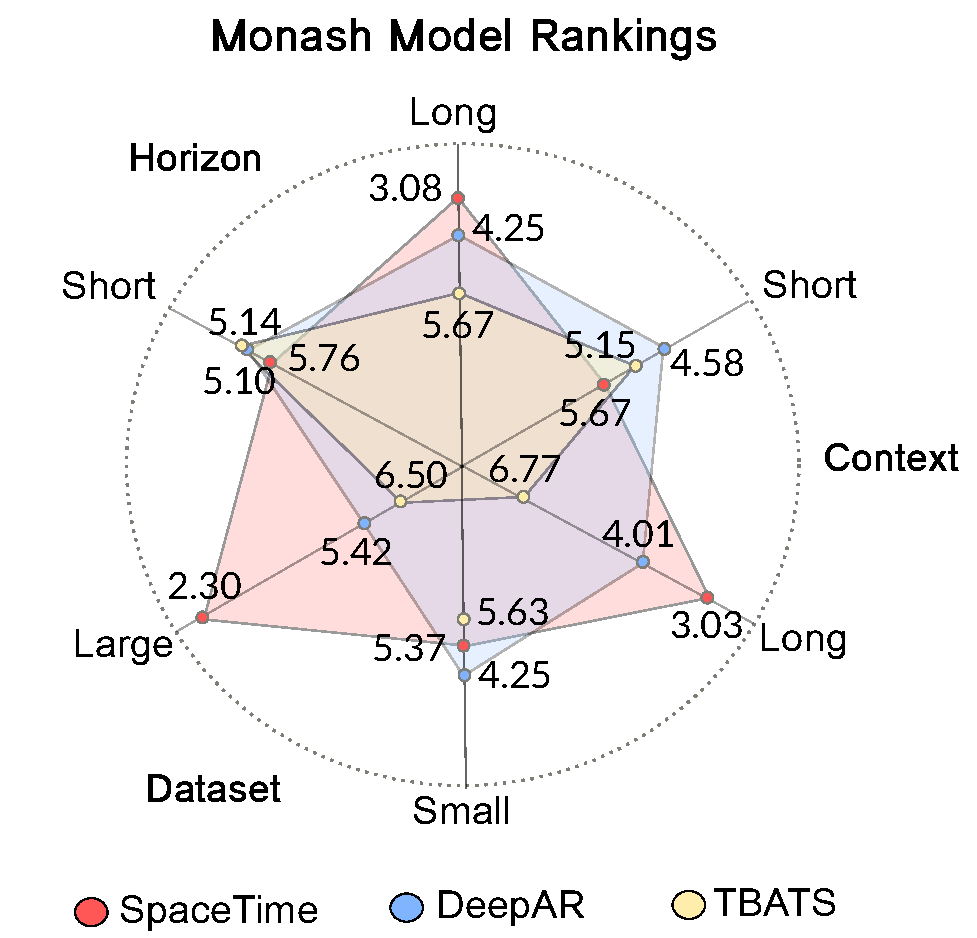
\includegraphics[width=\linewidth]{_ICLR2023_paper/figures/monash_rankings2.pdf}
%     \vspace{-0.4cm}
%     \caption{\footnotesize Relative test RMSE rankings ($*/12$ models) across different slices of the $33$ datasets in the Monash repository \citep{godahewa2021monash}. \ourmethod{} sets best overall ranking across all tasks and is significantly more accurate on tasks involving long forecast horizon and larger datasets.}
%     \label{fig:monash_rankings}
%     \vspace{-5cm}
% \end{wrapfigure}
%
% In Table~\ref{tab:informer-s-long}, we compare the standardized MSE and MAE of \ourmethod{} with that of recent state-of-the-art time series forecasting methods, related state-space models~\citep{gu2021efficiently}, and other competitive deep architectures. We also include ARIMA results as a classical approach baseline. 
We find \ourmethod{} obtains lowest MSE and MAE on 14 and 11 forecasting settings respectively, 3$\times$ more than prior state-of-the-art. \ourmethod{} also outperforms S4 on 15 / 16 settings, supporting the companion SSM representation.


\header{Monash (forecasting)} We also evaluate on $32$ datasets in the Monash forecasting benchmark
% Time Series Forecasting repository 
\citep{godahewa2021monash}, spanning domains including finance, weather, and traffic. For space, we report results in Table~\ref{tab:monash} (App.~\ref{app:monash_exps}). We compare against 13 classical and deep learning baselines.  
% , including classical (\eg{} SES \citep{winters1960forecasting})
% % , Theta \citep{assimakopoulos2000theta}), 
% and deep learning (\eg{} N-BEATS \citep{oreshkin2019n})
% % , Transformers \citep{vaswani2017attention})  
% % DeepAR \citep{salinas2020deepar}, 
% methods. 
\ourmethod{} achieves best RMSE on $7$ tasks and sets new state-of-the-art average performance across all $32$ datasets.
% , improving over both best classical and deep learning methods. 
% Furthermore, we find 
\ourmethod{}'s relative improvements also notably grow on long horizon tasks (Fig.~\ref{fig:monash_rankings}).
% analyze \ourmethod{}'s performance across task groups organized by forecasting horizon, dataset, and lag size. 
% we find \ourmethod{}'s relative gains notably grow with longer horizons and larger datasets. 
% \MZ{what is larger dataset?} 
% when the task involves longer forecasting horizons and a larger dataset.


\begin{table}[]
\caption{ \textbf{Univariate forecasting} results on Informer Electricity Transformer Temperature (ETT) datasets~\cite{zhou2021informer}. \textbf{Best} results in \textbf{bold}. \ourmethod{} results reported as means over three seeds. We include additional datasets, horizons, and method comparisons in App.~\ref{appendix:informer_extended}}
\resizebox{\linewidth}{!}{
\begin{tabular}{@{}c|cbcbcbcbcbcbcbcbc@{}}
\toprule
\multicolumn{2}{c}{Methods}                       & \multicolumn{2}{c}{SpaceTime}   & \multicolumn{2}{c}{NLinear}     & \multicolumn{2}{c}{FILM}        & \multicolumn{2}{c}{S4} & \multicolumn{2}{c}{FedFormer} & \multicolumn{2}{c}{Autoformer} & \multicolumn{2}{c}{Informer} & \multicolumn{2}{c}{ARIMA} \\ \midrule
\multicolumn{2}{c}{Metric}                        & MSE            & MAE            & MSE            & MAE            & MSE            & MAE            & MSE        & MAE       & MSE           & MAE           & MSE            & MAE           & MSE           & MAE          & MSE         & MAE         \\ \midrule
\parbox[t]{2mm}{\multirow{4}{*}{\rotatebox[origin=c]{90}{ETTh1}}} & 96  & 0.054          & 0.181          & \textbf{0.053} & \textbf{0.177} & 0.055          & 0.178          & 0.316      & 0.490     & 0.079         & 0.215         & 0.071          & 0.206         & 0.193         & 0.377        & 0.058       & 0.184       \\
\multicolumn{1}{c|}{}                       & 192 & \textbf{0.066} & 0.207          & 0.069          & \textbf{0.204} & 0.072          & 0.207          & 0.345      & 0.516     & 0.104         & 0.245         & 0.114          & 0.262         & 0.217         & 0.395        & 0.073       & 0.209       \\
\multicolumn{1}{c|}{}                       & 336 & \textbf{0.069} & \textbf{0.212} & 0.081          & 0.226          & 0.083          & 0.229          & 0.825      & 0.846     & 0.119         & 0.270         & 0.107          & 0.258         & 0.202         & 0.381        & 0.086       & 0.231       \\
\multicolumn{1}{c|}{}                       & 720 & \textbf{0.076} & \textbf{0.222} & 0.080          & 0.226          & 0.090          & 0.240          & 0.190      & 0.355     & 0.142         & 0.299         & 0.126          & 0.283         & 0.183         & 0.355        & 0.103       & 0.253       \\ \midrule
\parbox[t]{2mm}{\multirow{4}{*}{\rotatebox[origin=c]{90}{ETTh2}}} & 96  & \textbf{0.119} & \textbf{0.268} & 0.129          & 0.278          & 0.127          & 0.272          & 0.381      & 0.501     & 0.128         & 0.271         & 0.153          & 0.306         & 0.213         & 0.373        & 0.273       & 0.407       \\
\multicolumn{1}{c|}{}                       & 192 & \textbf{0.151} & \textbf{0.306} & 0.169          & 0.324          & 0.182          & 0.335          & 0.332      & 0.458     & 0.185         & 0.330         & 0.204          & 0.351         & 0.227         & 0.387        & 0.315       & 0.446       \\
\multicolumn{1}{c|}{}                       & 336 & \textbf{0.169} & \textbf{0.332} & 0.194          & 0.355          & 0.204          & 0.367          & 0.655      & 0.670     & 0.231         & 0.378         & 0.246          & 0.389         & 0.242         & 0.401        & 0.367       & 0.488       \\
\multicolumn{1}{c|}{}                       & 720 & \textbf{0.188} & \textbf{0.352} & 0.225          & 0.381          & 0.241          & 0.396          & 0.630      & 0.662     & 0.278         & 0.420         & 0.268          & 0.409         & 0.291         & 0.439        & 0.413       & 0.519       \\ \midrule
\parbox[t]{2mm}{\multirow{4}{*}{\rotatebox[origin=c]{90}{ETTm1}}} & 96  & \textbf{0.026} & \textbf{0.121} & \textbf{0.026} & 0.122          & 0.029          & 0.127          & 0.651      & 0.733     & 0.033         & 0.140         & 0.056          & 0.183         & 0.109         & 0.277        & 0.033       & 0.136       \\
\multicolumn{1}{c|}{}                       & 192 & \textbf{0.039} & 0.152          & \textbf{0.039} & \textbf{0.149} & 0.041          & 0.153          & 0.190      & 0.372     & 0.058         & 0.186         & 0.081          & 0.216         & 0.151         & 0.310        & 0.049       & 0.169       \\
\multicolumn{1}{c|}{}                       & 336 & \textbf{0.051} & 0.173          & 0.052          & \textbf{0.172} & 0.053          & 0.175          & 0.428      & 0.581     & 0.084         & 0.231         & 0.076          & 0.218         & 0.427         & 0.591        & 0.065       & 0.196       \\
\multicolumn{1}{c|}{}                       & 720 & 0.074          & 0.213          & 0.073          & 0.207          & \textbf{0.071} & \textbf{0.205} & 0.254      & 0.433     & 0.102         & 0.250         & 0.110          & 0.267         & 0.438         & 0.586        & 0.089       & 0.231       \\ \midrule
\parbox[t]{2mm}{\multirow{4}{*}{\rotatebox[origin=c]{90}{ETTm2}}} & 96  & \textbf{0.060} & \textbf{0.179} & 0.063          & 0.182          & 0.065          & 0.189          & 0.153      & 0.318     & 0.067         & 0.198         & 0.065          & 0.189         & 0.088         & 0.225        & 0.211       & 0.340       \\
\multicolumn{1}{c|}{}                       & 192 & \textbf{0.090} & \textbf{0.222} & \textbf{0.090} & 0.223          & 0.094          & 0.233          & 0.183      & 0.350     & 0.102         & 0.245         & 0.118          & 0.256         & 0.132         & 0.283        & 0.237       & 0.371       \\
\multicolumn{1}{c|}{}                       & 336 & \textbf{0.113} & \textbf{0.255} & 0.117          & 0.259          & 0.124          & 0.274          & 0.204      & 0.367     & 0.130         & 0.279         & 0.154          & 0.305         & 0.180         & 0.336        & 0.264       & 0.396       \\
\multicolumn{1}{c|}{}                       & 720 & \textbf{0.166} & \textbf{0.318} & 0.170          & 0.318          & 0.173          & 0.323          & 0.482      & 0.567     & 0.178         & 0.325         & 0.182          & 0.335         & 0.300         & 0.435        & 0.310       & 0.441       \\ \midrule
\multicolumn{2}{c}{Count}                         & \textbf{14}    & \textbf{11}    & 4              & 4              & 1              & 1              & 0          & 0         & 0             & 0             & 0              & 0             & 0             & 0            & 0           & 0           \\ \bottomrule
\end{tabular}
% \begin{tabular}{@{}c|cbcbcbcbcbcbcbcbcac@{}}
% \toprule
% \multicolumn{2}{c}{Methods}                       & \multicolumn{2}{c}{\textbf{\ourmethod{}}}   & \multicolumn{2}{c}{NLinear}     & \multicolumn{2}{c}{FILM} & \multicolumn{2}{c}{S4} & \multicolumn{2}{c}{FedFormer} & \multicolumn{2}{c}{SCINet} & \multicolumn{2}{c}{Autoformer} & \multicolumn{2}{c}{Informer} & \multicolumn{2}{c}{ARIMA} \\ \midrule
% \multicolumn{2}{c}{Metric}                        & MSE            & MAE            & MSE            & MAE            & MSE         & MAE        & MSE        & MAE       & MSE           & MAE           & MSE          & MAE         & MSE            & MAE           & MSE           & MAE          & MSE         & MAE         \\ \midrule
% % \multicolumn{1}{c|}{\multirow{4}{*}{ETTh1}} 
% \parbox[t]{2mm}{\multirow{4}{*}{\rotatebox[origin=c]{90}{ETTh1}}}
% & 96  & 0.054          & 0.181          & \textbf{0.053} & \textbf{0.177} & 0.055       & 0.178      & 0.316*          & 0.490*         & 0.079         & 0.215         & -            & -           & 0.071          & 0.206         & 0.193         & 0.377        & -           & -           \\
% \multicolumn{1}{c|}{}                       & 192 & 0.070          & 0.210          & \textbf{0.069} & \textbf{0.204} & 0.072       & 0.207      & 0.345* & 0.516*       & 0.104         & 0.245         & -            & -           & 0.114          & 0.262         & 0.217         & 0.395        & -           & -           \\
% \multicolumn{1}{c|}{}                       & 336 & \textbf{0.070} & \textbf{0.213} & 0.081          & 0.226          & 0.083       & 0.229      & 0.080      & 0.229     & 0.119         & 0.270         & 0.094        & 0.242       & 0.107          & 0.258         & 0.202         & 0.381        & 0.468       & 0.593       \\
% \multicolumn{1}{c|}{}                       & 720 & \textbf{0.076} & \textbf{0.222} & 0.080          & 0.226          & 0.090       & 0.240      & 0.116      & 0.271     & 0.142         & 0.299         & 0.176        & 0.343       & 0.126          & 0.283         & 0.183         & 0.355        & 0.659       & 0.766       \\ \midrule
% % \multicolumn{1}{c|}{\multirow{4}{*}{ETTh2}} 
% \parbox[t]{2mm}{\multirow{4}{*}{\rotatebox[origin=c]{90}{ETTh2}}}
% & 96  & \textbf{0.119} & \textbf{0.267} & 0.129          & 0.278          & 0.127       & 0.272      & 0.381* & 0.501*         & 0.128         & 0.271         & -            & -           & 0.153          & 0.306         & 0.213         & 0.373        & -           & -           \\
% \multicolumn{1}{c|}{}                       & 192 & \textbf{0.090} & \textbf{0.222} & \textbf{0.090} & 0.223          & 0.094       & 0.233      & 0.332* & 0.458*        & 0.102         & 0.245         & -            & -           & 0.118          & 0.256         & 0.132         & 0.283        & -           & -           \\
% \multicolumn{1}{c|}{}                       & 336 & \textbf{0.169} & \textbf{0.332} & 0.194          & 0.355          & 0.204       & 0.367      & 0.189      & 0.361     & 0.231         & 0.378         & 0.177        & 0.340       & 0.246          & 0.389         & 0.242         & 0.401        & 2.753       & 0.738       \\
% \multicolumn{1}{c|}{}                       & 720 & 0.188 & \textbf{0.352} & 0.225          & 0.381          & 0.241       & 0.396      & \textbf{0.187}      & 0.358     & 0.278         & 0.420         & 0.253        & 0.403       & 0.268          & 0.409         & 0.291         & 0.439        & 2.878       & 1.044       \\ \midrule
% % \multicolumn{1}{c|}{\multirow{4}{*}{ETTm1}} 
% \parbox[t]{2mm}{\multirow{4}{*}{\rotatebox[origin=c]{90}{ETTm1}}}
% & 96  & \textbf{0.026} & \textbf{0.121} & \textbf{0.026} & 0.122          & 0.029       & 0.127      & 0.086      & 0.229     & 0.033         & 0.140         & 0.072        & 0.198       & 0.056          & 0.183         & 0.109         & 0.277        & 0.272       & 0.399       \\
% \multicolumn{1}{c|}{}                       & 192 & \textbf{0.039} & 0.152          & \textbf{0.039} & \textbf{0.149} & 0.041       & 0.153      & 0.190* & 0.372*          & 0.058         & 0.186         & -            & -           & 0.081          & 0.216         & 0.151         & 0.310        & -           & -           \\
% \multicolumn{1}{c|}{}                       & 336 & \textbf{0.051} & 0.173          & 0.052          & \textbf{0.172} & 0.053       & 0.175      &    0.428* & 0.581*      & 0.084         & 0.231         & -            & -           & 0.076          & 0.218         & 0.427         & 0.591        & -           & -           \\
% \multicolumn{1}{c|}{}                       & 720 & 0.074          & 0.213          & 0.073 & 0.207 & \textbf{0.071}       & \textbf{0.205}      & 0.254* & 0.433*        & 0.102         & 0.250         & -            & -           & 0.110          & 0.267         & 0.438         & 0.586        & -           & -           \\ \midrule
% % \multicolumn{1}{c|}{\multirow{4}{*}{ETTm2}} 
% \parbox[t]{2mm}{\multirow{4}{*}{\rotatebox[origin=c]{90}{ETTm2}}}
% & 96  & \textbf{0.060} & \textbf{0.179} & 0.063          & 0.182          & 0.065       & 0.189      & 0.153* & 0.318*        & 0.067         & 0.198         & -            & -           & 0.065          & 0.189         & 0.088         & 0.225        & -           & -           \\
% \multicolumn{1}{c|}{}                       & 192 & \textbf{0.090} & \textbf{0.222} & \textbf{0.090} & 0.223          & 0.094       & 0.233      &  0.183* & 0.350*         & 0.102         & 0.245         & -            & -           & 0.118          & 0.256         & 0.132         & 0.283        & -           & -           \\
% \multicolumn{1}{c|}{}                       & 336 & \textbf{0.113} & \textbf{0.255} & 0.117          & 0.259          & 0.124       & 0.274      & 0.204* & 0.367*         & 0.130         & 0.279         & -            & -           & 0.154          & 0.305         & 0.180         & 0.336        & -           & -           \\
% \multicolumn{1}{c|}{}                       & 720 & \textbf{0.166} & \textbf{0.318} & 0.170          & 0.318          & 0.173       & 0.323      & 0.482* & 0.567*        & 0.178         & 0.325         & -            & -           & 0.182          & 0.335         & 0.300         & 0.435        & -           & -           \\ \midrule
% \multicolumn{2}{c}{Count}                         & \textbf{12}    & \textbf{11}    & 6              & 4              & 1           & 1          & 1          & 0         & 0             & 0             & 0            & 0           & 0              & 0             & 0             & 0            & 0           & 0           \\ \bottomrule
% \end{tabular}
}
\label{tab:informer-s-long}
\end{table}

%
\begin{table}[!t]
% \begin{minipage}[c]{0.745\textwidth}
\begin{minipage}[c]{0.7\textwidth}
\centering
\captionof{table}{ \textbf{ECG statement classification} on PTB-XL (100 Hz version). Baseline AUROC from \cite{strodthoff2021benchmarking} (error bars in App. \ref{appendix:ecg_results}).
}
\resizebox{1\linewidth}{!}{
% \small
\begin{tabular}{@{}lcccccc@{}}
\toprule
Task AUROC & All            & Diag           & Sub-diag       & Super-diag     & Form           & Rhythm         \\ \midrule
\textbf{\ourmethod{}}            & {\ul 0.936}    & \textbf{0.941} & \textbf{0.933} & {\ul 0.929} & 0.883          & {\ul 0.967}    \\
{\ul S4  }                 & \textbf{0.938} & {\ul 0.939}    & 0.929          & \textbf{0.931}    & 0.895          & \textbf{0.977} \\
Inception-1D         & 0.925          & 0.931          & {\ul 0.930}    & 0.921          & \textbf{0.899} & 0.953          \\
xRN-101              & 0.925          & 0.937          & 0.929          & 0.928   & {\ul 0.896}    & 0.957          \\
LSTM                 & 0.907          & 0.927          & 0.928          & 0.927          & 0.851          & 0.953          \\
Transformer         & 0.857          & 0.876          & 0.882    & 0.887          & 0.771 & 0.831          \\
Wavelet + NN         & 0.849          & 0.855          & 0.859          & 0.874          & 0.757          & 0.890          \\ \bottomrule
\end{tabular}
}
\label{tab:ptbxl_100}
\end{minipage}
\quad
% \begin{minipage}[c]{0.2225\textwidth}
\begin{minipage}[c]{0.23\textwidth}
\centering
\captionof{table}{\textbf{Speech Audio classification}~\citep{warden2018speech}
% on raw 16,000 time-step)
}

\resizebox{1\linewidth}{!}{
\begin{tabular}{@{}lc@{}}
\toprule
Method      & Acc. (\%)         \\ \midrule
 \ourmethod{}   & {\ul 97.29}           \\
S4         & \textbf{98.32}        \\
\textsc{LSSL}        & \xmark \\
WaveGan-D   & 96.25                 \\
Transformer & \xmark \\
Performer   & 30.77                 \\
CKConv      & 71.66                 \\ \bottomrule
\end{tabular}
}
\label{tab:speech_commands}
\end{minipage}
% \vspace{-0.75cm}
\end{table}

\header{ECG (multi-label classification)} Beyond forecasting, we show that \ourmethod{} can also perform state-of-the-art time series classification. To classify sequences, we use the same sequence model architecture in Sec.~\ref{sec:expressive_ssm_layer}. Like prior work~\citep{gu2021efficiently}, we simply use the last-layer FFN to project from number of SSMs to number of classes, and mean pooling over length before a softmax to output class logits. 
%
In Table~\ref{tab:ptbxl_100}, we find that \ourmethod{} obtains best or second-best AUROC on five out of six tasks, outperforming both general sequence models and specialized architectures. 

\header{Speech Audio (single-label classification)} We further test \ourmethod{} on long-range audio classification on the Speech Commands dataset \citep{warden2018speech}. The task is classifying raw audio sequences of length 16,000 into 10 word classes.
%reporting accuracy (Acc.) on classifying sequences up to 16,000 time-steps long. 
We use the same pooling operation for classification as in ECG. \ourmethod{} outperforms domain-specific architectures, \eg{} WaveGan-D~\citep{donahue2018adversarial}  and efficient Transformers, \eg{} Performer~\citep{choromanski2020rethinking} (Table~\ref{tab:speech_commands}).
% \ourmethod{} outperforms prior SSMs (LSSL), Transformers, and specialized architectures (Table~\ref{tab:speech_commands}). 

%


% We consider two forecasting benchmark archives: 

% \begin{itemize}[leftmargin=*]
%     \item \textbf{Informer} \citep{zhou2021informer}: The long sequence forecasting tasks come from three time series datasets: ETT, which are time series representing the temperatures of electricity transformers~\tempcite{}, ECL, which represents the electricity consumption of 321 clients, and Weather, which represents local climatological data of around $1{,}600$ locations collected hourly over the span of four years~\tempcite{}. Three forecasting tasks were created from ETT, two tasks are collected hourly from two counties in China (ETTh1 and ETTh2), and one task is collected at a 15-minute cadence (ETTm1).
%     \item \textbf{Monash}  \citep{godahewa2021monash}: Monash contains $30$ time series datasets with different forecasting settings, such as the frequency of the collected data (e.g., hourly or yearly), the context length, the forecasting horizon, and uni/multi-variate data. The datasets span a broad range of domains, including energy, tourism, sales, banking, transportation, and more. Since multiple time series tasks can be defined from each dataset (e.g., varying the frequency of the data), Monash comprises a total $58$ time series forecasting tasks. 
% \end{itemize}

% For all forecasting tasks, we validate our hypothesis that \ourmethod{} is broadly applicable to diverse settings by comparing its performance with a number of both classical time series methods, along with more recent deep learning approaches. For classical approaches, we report the forecasting performance of ARIMA and ETS models that have been fitted to each task in previous work \citep{zhou2021informer,godahewa2021monash}. For deep learning approaches, we compare to specialized transformer-based architectures, such as  FiLM~\citep{zhou2022film}, ETSFormer~\tempcite{}, and AutoFormer~\citep{wu2021autoformer}, along with simpler, yet high-performing, methods such as DLinear \citep{zeng2022transformers}, and finally, other deep SSM-based methods such as S4 \citep{gu2021efficiently}.

%On the Monash benchmark, we compare the average Root Mean Squared Error (RMSE) to $12$ methods, which include traditional and modern deep learning methods \citep{godahewa2021monash}. On the long sequence forecasting tasks, we compare the average Mean Squared Error (MSE) and Mean Absolute Error (MAE) of \ourmethod{} to ETSFormer~\tempcite{}, AutoFormer~\tempcite{}, Informer~\tempcite{}, DeepAR~\tempcite{}, and ARIMA~\tempcite{}.





\subsection{Improvement on Criteria for Effective Time Series Modeling} 
\label{sec:empirical_claims}

For further insight into \ourmethod{}'s performance, we now validate that our contributions improve expressivity (\ref{sec:empirical_expressivity}), forecasting ability (\ref{sec:empirical_horizons}), and efficiency (\ref{sec:empirical_efficiency}) over existing approaches. 

% empirically validate the design choices of \ourmethod{}, and showcase the advantage of (i) the companion matrix in improving expressivity, (ii) the closed-loop SSM in it's ability to generalize to arbitrary forecast horizons, and (iii) the efficiency in processing long sequences.

\subsubsection{Expressivity} \label{sec:empirical_expressivity}
% \vspace{-0.125cm}

To first study \ourmethod{}'s expressivity, we test how well \ourmethod{} can fit controlled autoregressive processes. 
% We use the simplest version of \ourmethod{}, which reduces to a single linear layer with weights parameterizing one companion SSM.
%
To validate our theory on \ourmethod{}'s expressivity gains in Sec.~\ref{sec:expressive_ssm_layer}, we compare against recent related SSM architectures such as S4~\citep{gu2021efficiently} and S4D~\citep{gu2022parameterization}. 

For evaluation, we generate noiseless synthetic AR($p$) sequences. 
% Knowing the true coefficients,
% behind each time series process. Beyond forecasting accuracy, 
We test if models learn the true process by inspecting whether the trained model weights recover \emph{transfer functions} specified by the AR coefficients~\citep{oppenheim1999discrete}. 
% To test if parameterized SSMs \emph{can express} the true processes, 
We use simple 1-layer 1-SSM models, with state-space size equal to AR $p$, and predict one time-step given $p$ lagged inputs (the smallest sufficient setting).

In Fig.~\ref{fig:arima_synthetics} we compare the trained forecasts and transfer functions (as frequency response plots) of \ourmethod{}, S4, and S4D models on a relatively smooth AR(4) process and sharp AR(6) process. Our results support the relative expressivity of \ourmethod{}'s companion matrix SSM. While all models accurately forecast the AR(4) time series, only \ourmethod{} recovers the ground-truth transfer functions for both, and notably forecasts the AR(6) process more accurately (Fig.~\ref{fig:arima_synthetics}c, d). 

% \begin{figure}[ht]
\begin{figure}[!t]
\centering
\subfigure[ AR(4) Forecast]{
    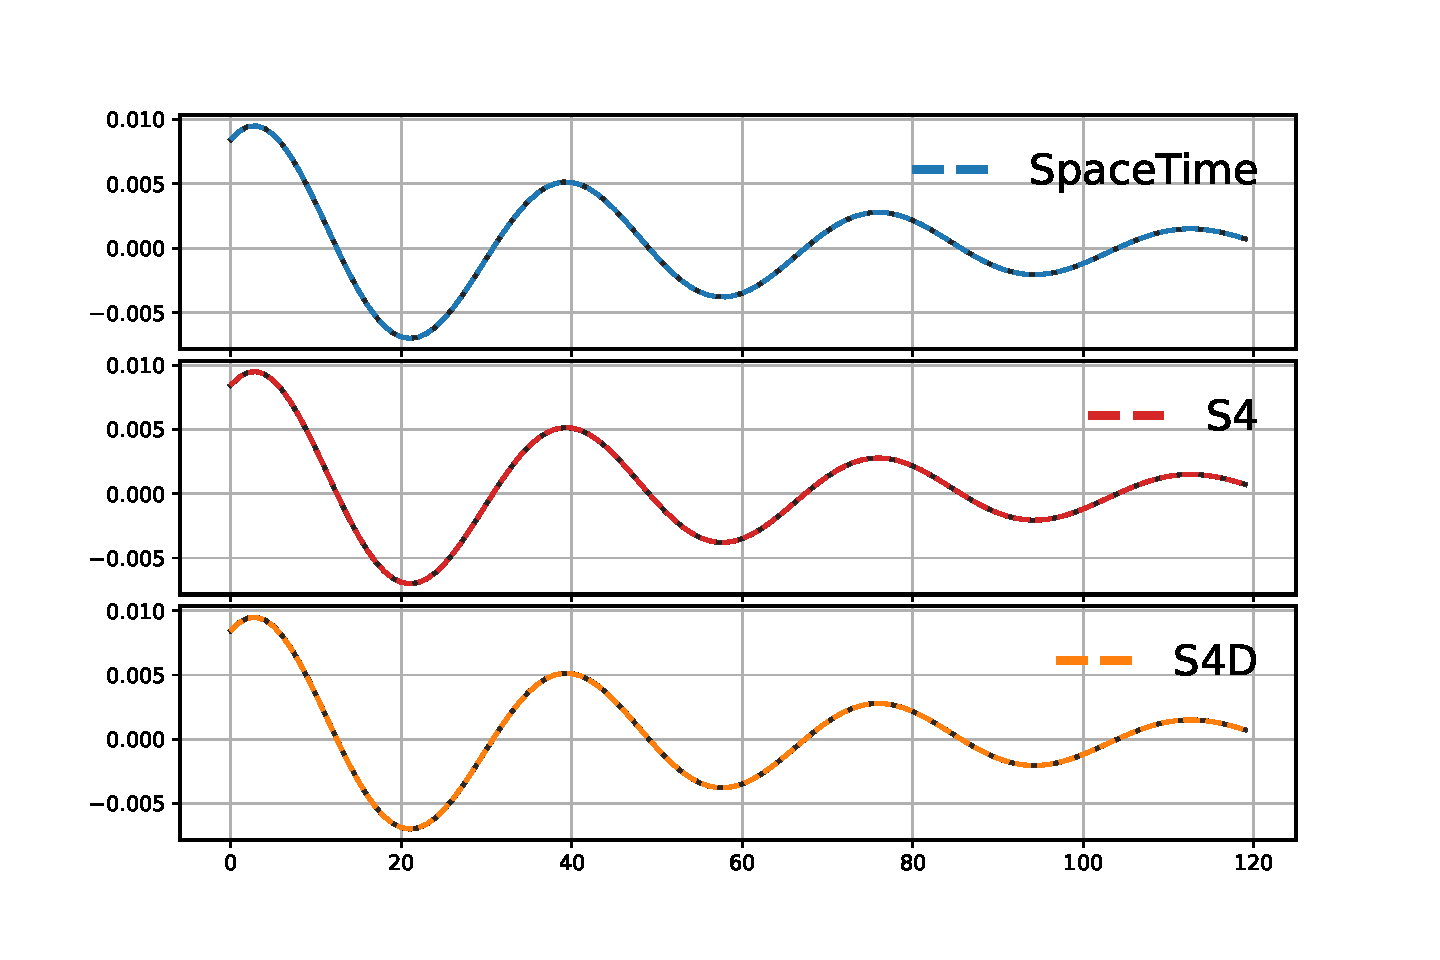
\includegraphics[width=0.22\textwidth]{_ICLR2023_paper/figures/arima_synthetic-ar_4-forecasts-wider-rmse.pdf}
    \label{fig:arima_synthetic_ar_4_forecast}
}
\subfigure[ AR(4) Transfer Func.]{
    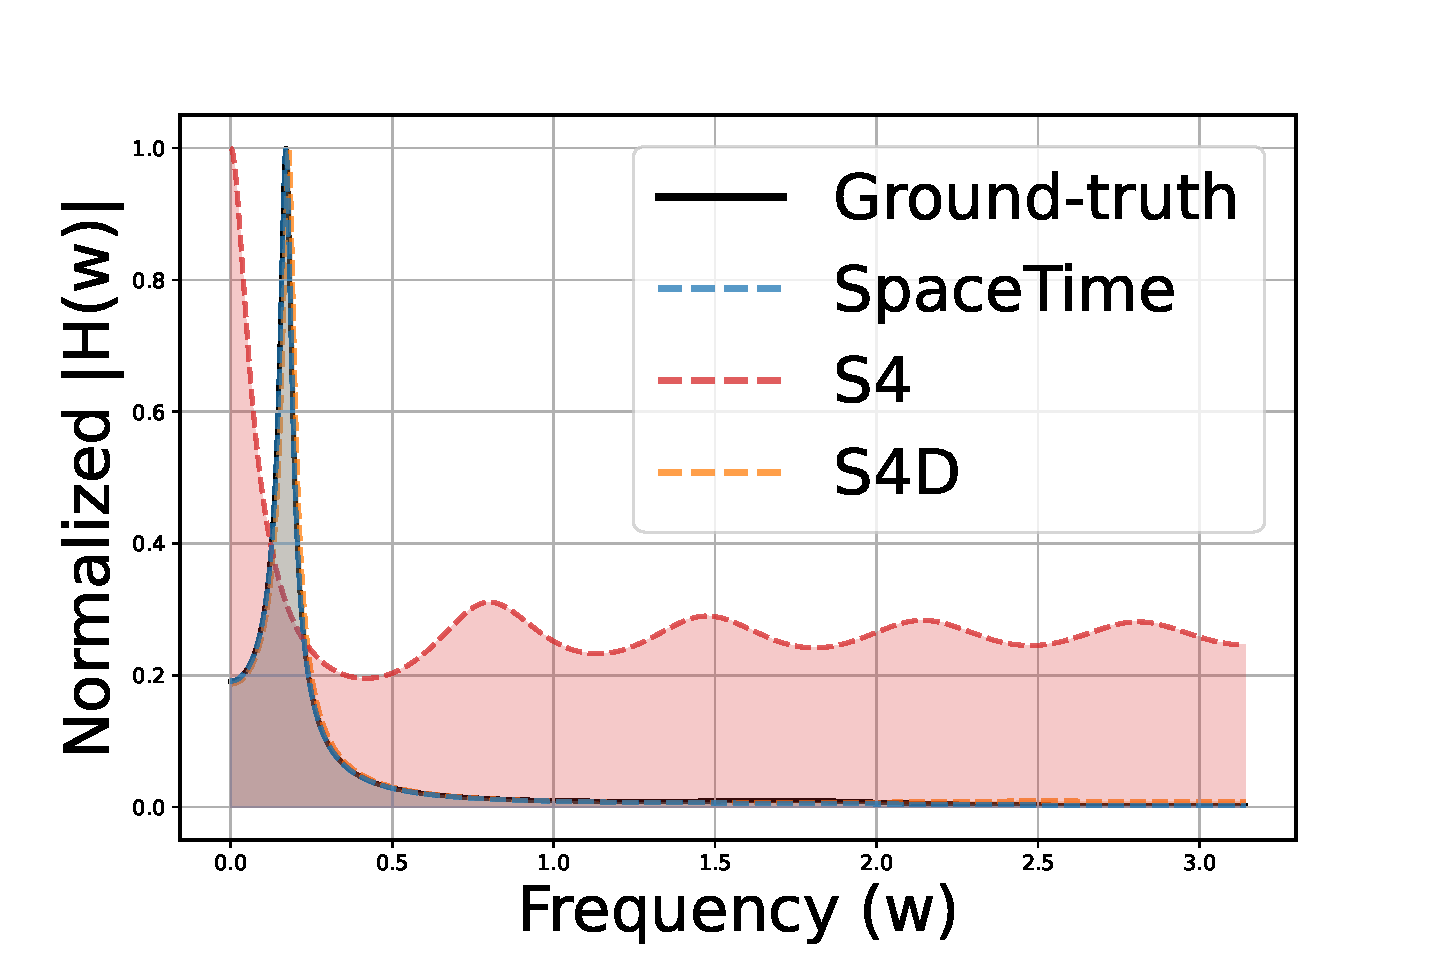
\includegraphics[width=0.22\textwidth]{_ICLR2023_paper/figures/arima_synthetic-ar_4-freq_response-seed=0-wider-rmse.pdf}
    \label{fig:arima_synthetic_ar_4_transfer}
}
\subfigure[ AR(6) Forecast]{
    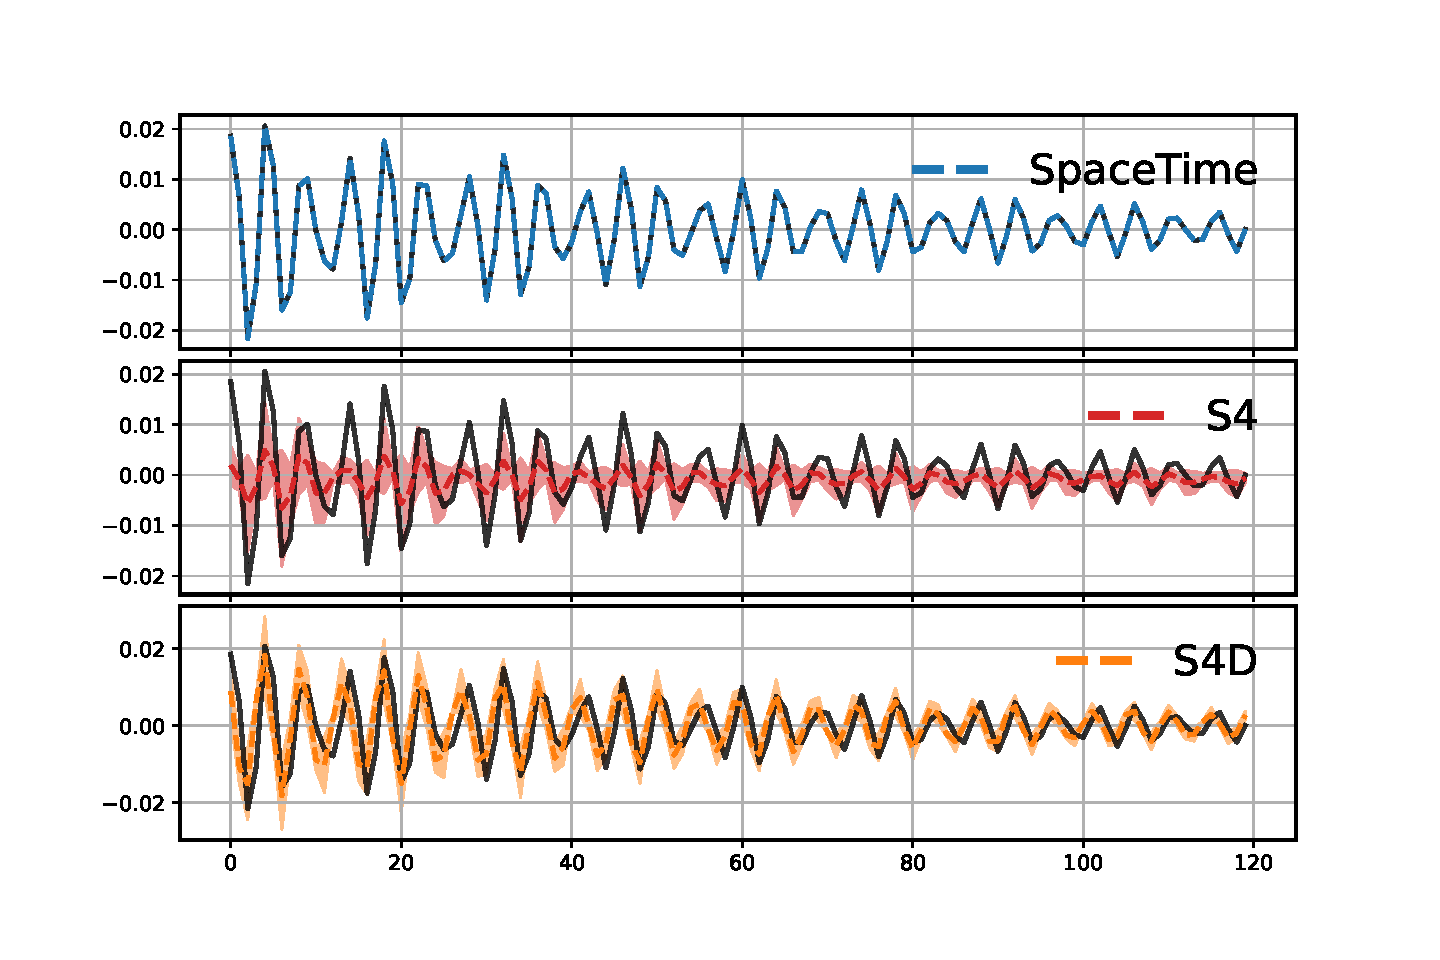
\includegraphics[width=0.22\textwidth]{_ICLR2023_paper/figures/arima_synthetic-ar_6-forecasts-wider-rmse.pdf}
    \label{fig:arima_synthetic_ar_6_forecast}
}
\subfigure[ AR(6) Transfer Func.]{
    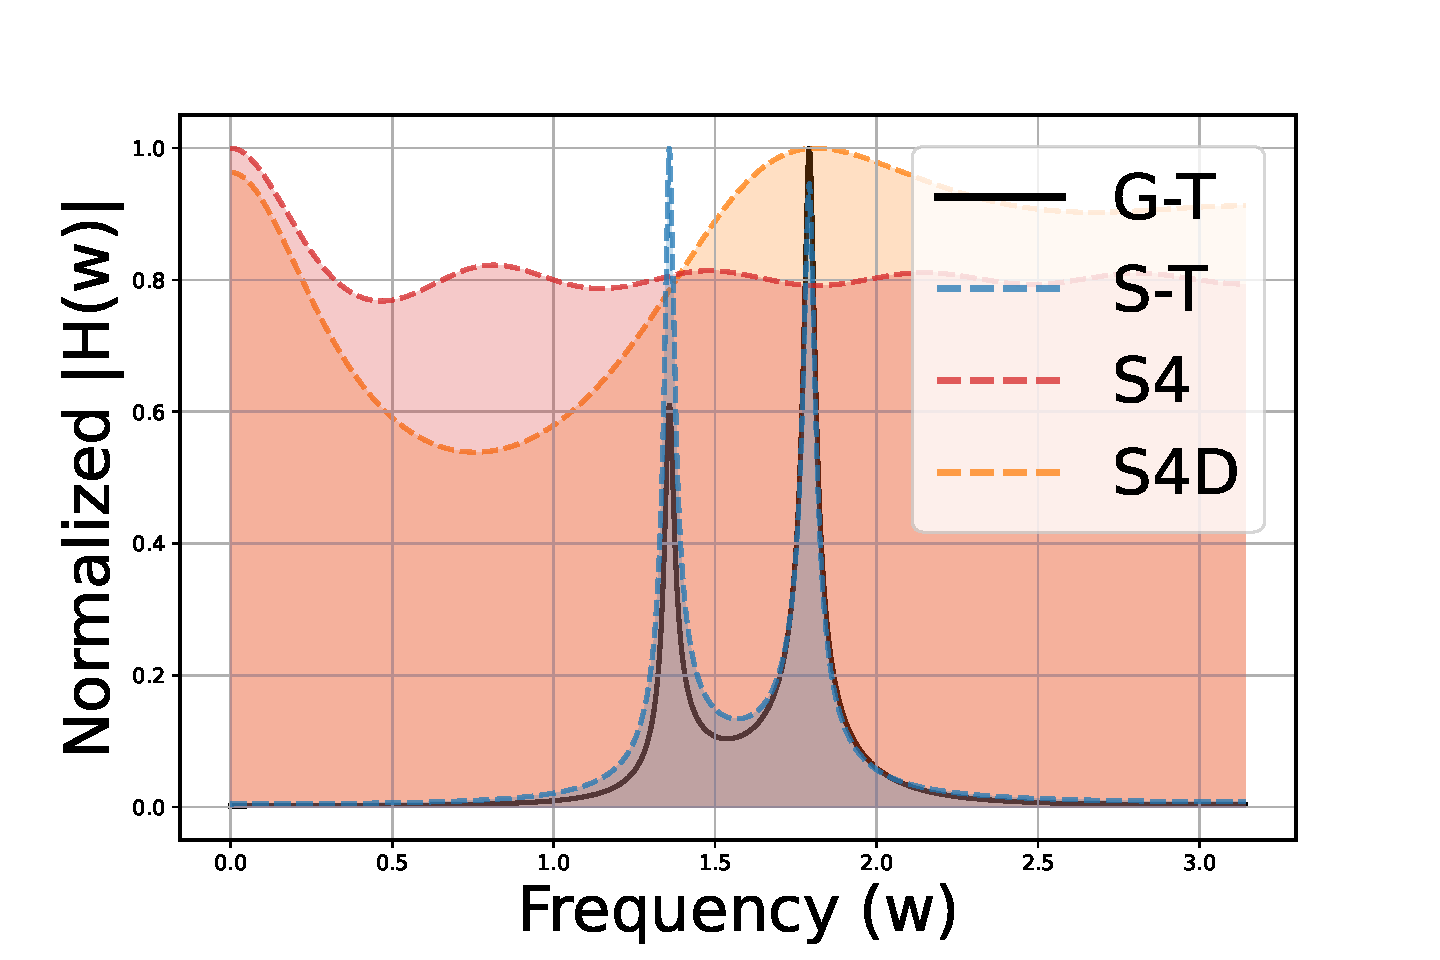
\includegraphics[width=0.22\textwidth]{_ICLR2023_paper/figures/arima_synthetic-ar_6-freq_response-seed=0-wider-rmse.pdf}
    \label{fig:arima_synthetic_ar_6_transfer}
}
\caption{ \textbf{AR($p$) expressiveness benchmarks}. \ourmethod{} captures AR($p$) processes more precisely than similar deep SSM models such as S4~\cite{gu2021efficiently} and S4D~\cite{gu2022parameterization}, forecasting future samples and learning ground-truth transfer functions more accurately.}
\label{fig:arima_synthetics}
\end{figure}


% \begin{figure}[H]
% \centering
% \begin{subfigure}
% \centering
%     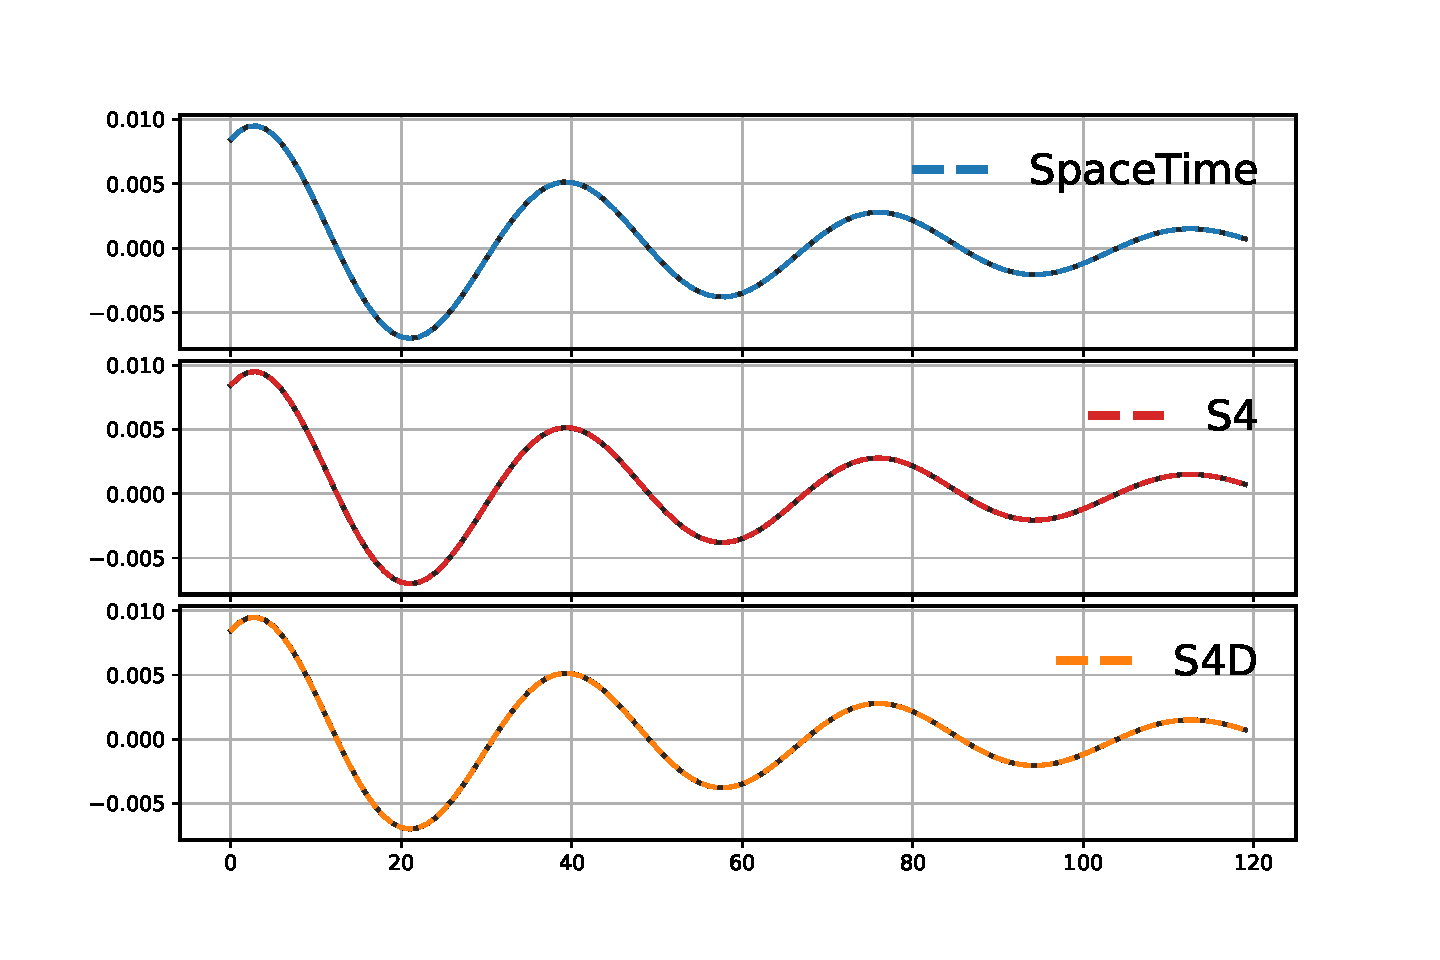
\includegraphics[width=0.2\linewidth]{_ICLR2023_paper/figures/arima_synthetic-ar_4-forecasts-wider-rmse.pdf}
%     \caption{\small AR(4) Forecast}
%     \label{fig:arima_synthetic_ar_4}
% \end{subfigure}
% \begin{subfigure}
% \centering
%     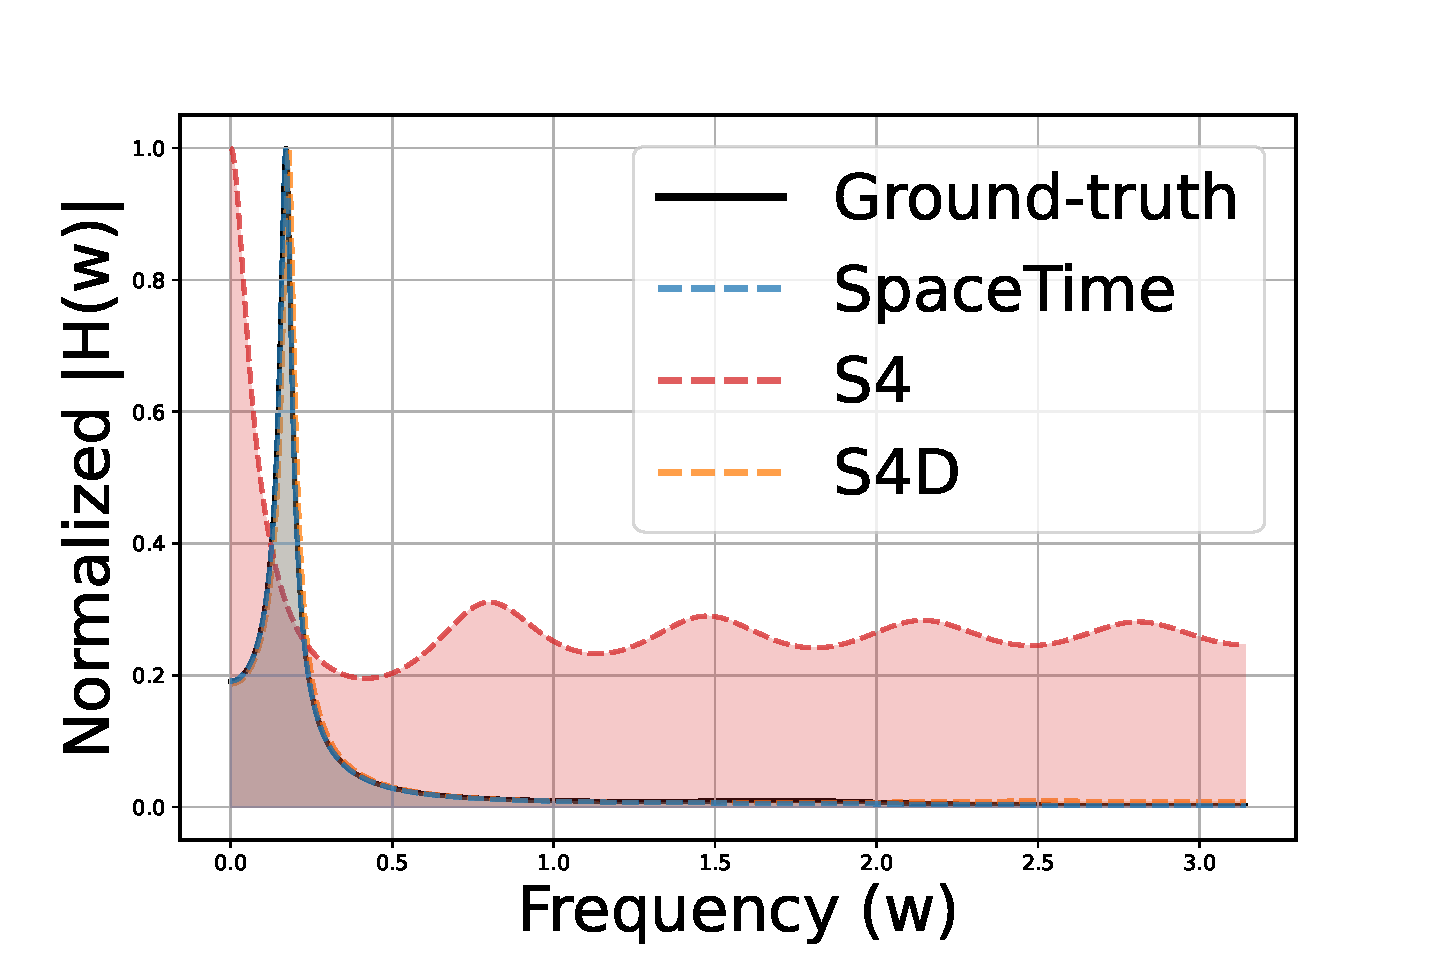
\includegraphics[width=0.2\linewidth]{_ICLR2023_paper/figures/arima_synthetic-ar_4-freq_response-seed=0-wider-rmse.pdf}
%     \caption{\small AR(4) Transfer Func.}
%     \label{fig:arima_synthetic_ar_4}
% \end{subfigure}
% \begin{subfigure}
% \centering
%     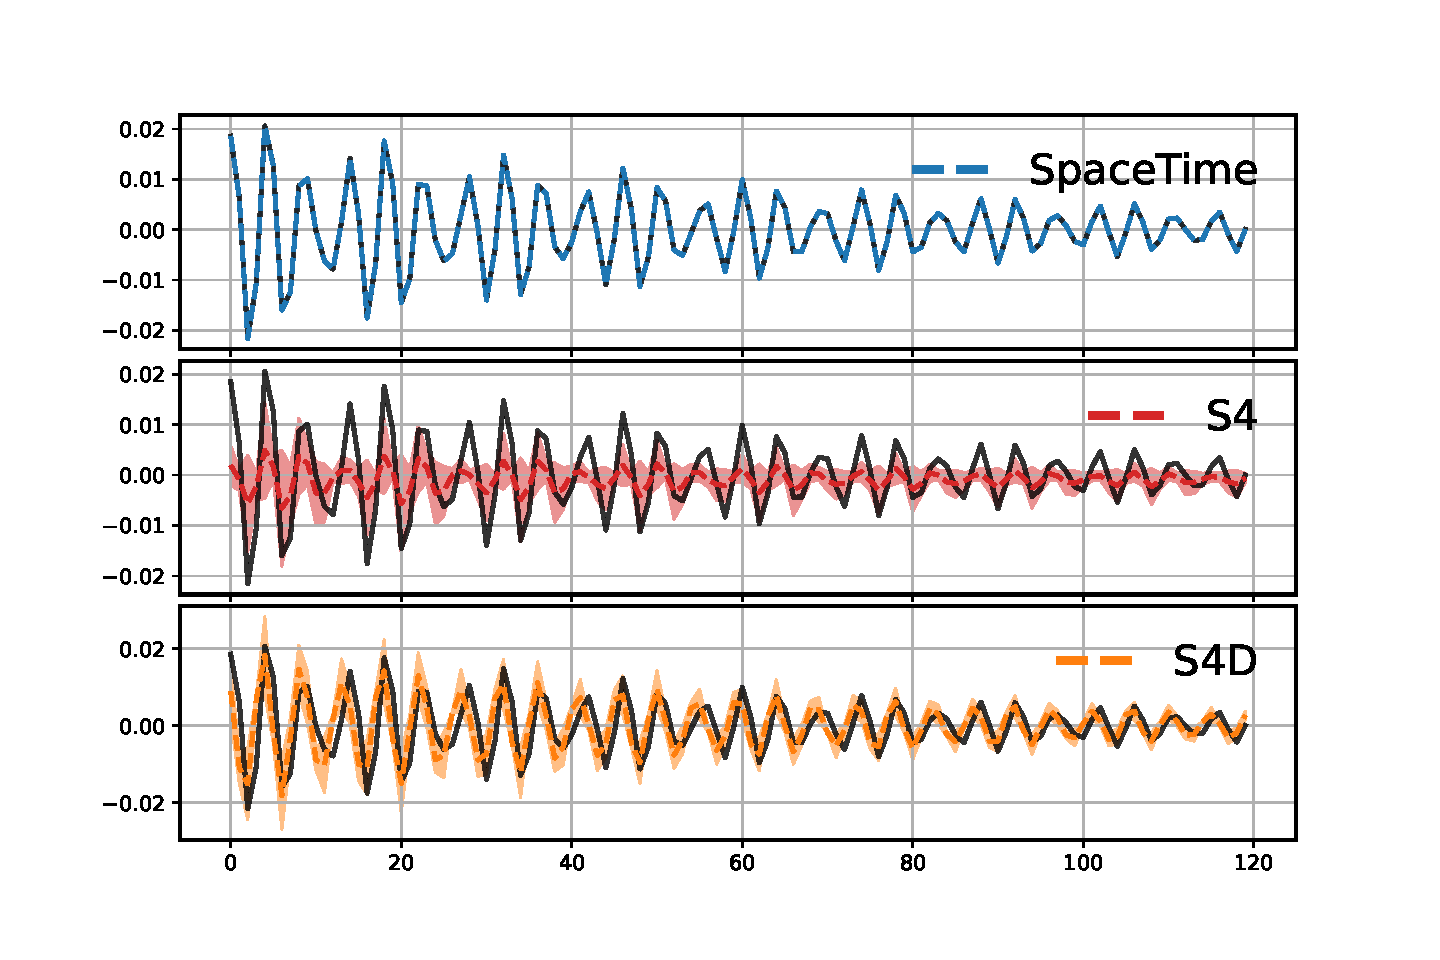
\includegraphics[width=0.2\linewidth]{_ICLR2023_paper/figures/arima_synthetic-ar_6-forecasts-wider-rmse.pdf}
%     \caption{\small AR(6) Forecast}
%     \label{fig:arima_synthetic_ar_6}
% \end{subfigure}
% \begin{subfigure}
% \centering
%     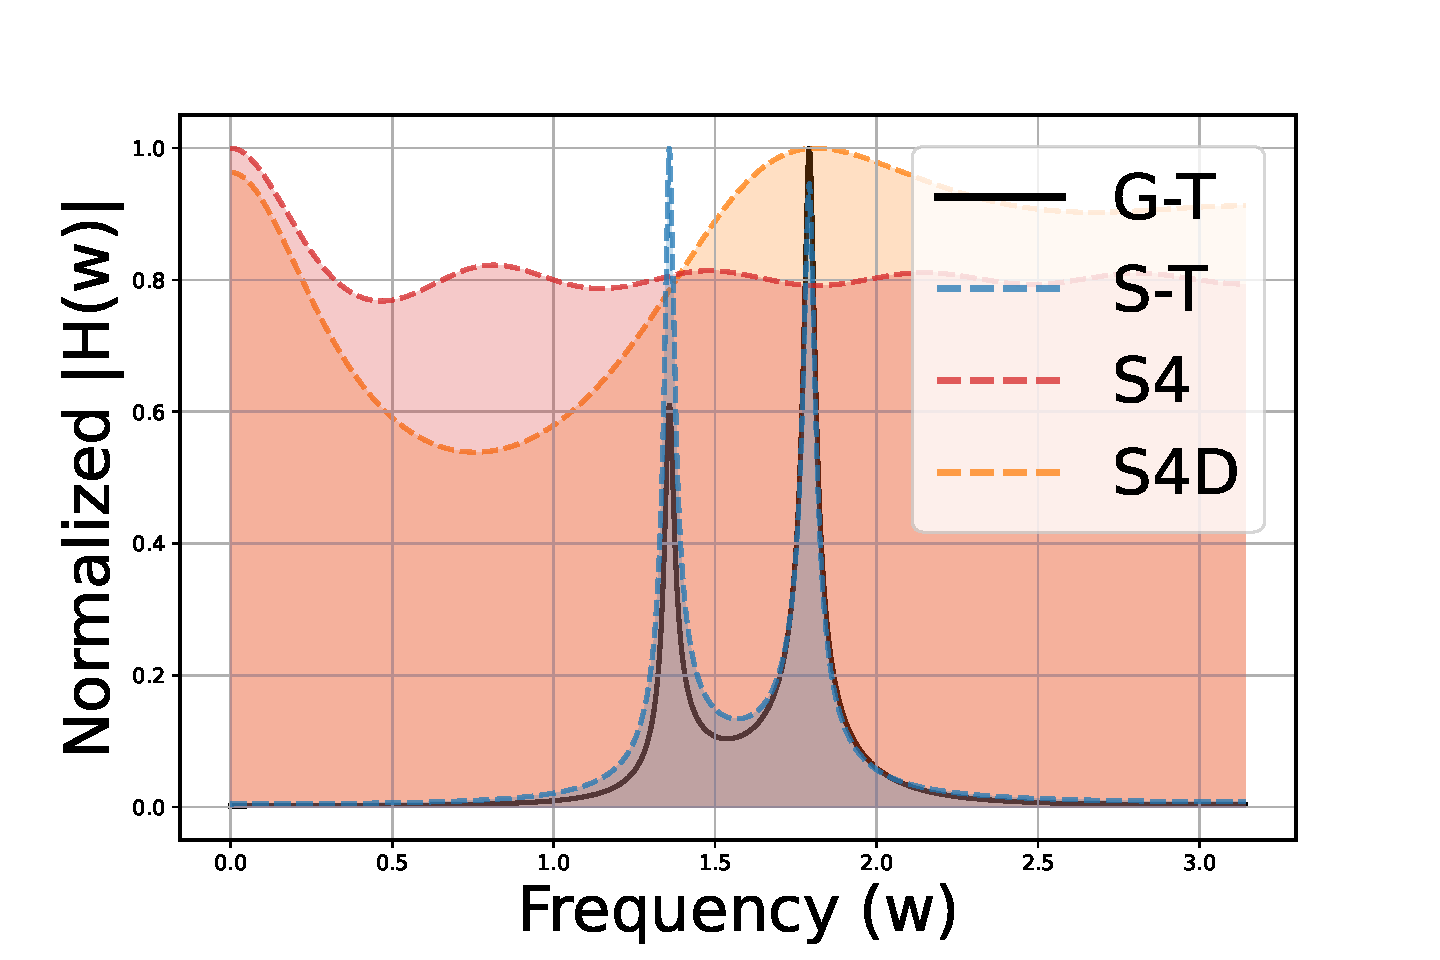
\includegraphics[width=0.2\linewidth]{_ICLR2023_paper/figures/arima_synthetic-ar_6-freq_response-seed=0-wider-rmse.pdf}
%     \caption{\small AR(6) Transfer Func.}
%     \label{fig:arima_synthetic_ar_6}
% \end{subfigure}
% \caption{\small \textbf{AR($p$) expressiveness benchmarks}. \ourmethod{} captures AR processes more precisely than similar deep SSM models, forecasting future samples and learning ground-truth transfer functions more accurately.}
% \label{fig:arima_synthetics}
% \end{figure}

% \begin{figure}[H]
\begin{figure}[!t]
% \vspace{-0.25cm}
\begin{minipage}[c]{0.55\textwidth}
\centering
\captionof{table}{ \textbf{Longer horizon forecasting} on Informer ETTh data. Standardized MSE reported. \ourmethod{} obtains lower MSE when forecasting longer horizons.}\label{tab:long_horizon_etth}
\resizebox{1\linewidth}{!}{
\tabcolsep=0.1cm
  \begin{tabular}{@{}llcccccc@{}}
\toprule
Dataset & Horizon & 720            & 960            & 1080                  & 1440           & 1800                  & 1920                  \\ \midrule
\multirow{2}{*}{ETTh1}      & NLinear                    & 0.080          & 0.089         & 0.085                & 0.094          & 0.102 & 0.104 \\
                            & \ourmethod{}                  & \textbf{0.075} & \textbf{0.074} & \textbf{0.072}        & \textbf{0.080} & \textbf{0.081}        & \textbf{0.088}        \\
                            % & Rel. Improve.              & 0.056          & 0.279          & 0.127                 & 0.390          & -                     & -                     \\ 
                            \midrule
\multirow{2}{*}{ETTh2}      & NLinear                    & 0.224          & 0.273          & 0.290 & 0.329          & 0.450               & 0.493 \\
                            & \ourmethod{}                  & \textbf{0.188} & \textbf{0.225} & \textbf{0.265}        & \textbf{0.299} & 
                            % 0.541
                            \textbf{0.438}
                            & \textbf{0.459}        \\
                            % & Rel. Improve.              & 0.506          & 0.457          & -                     & 0.361          & 0.968                 & -                     \\ 
                            \bottomrule
\end{tabular}
}
\end{minipage}
\quad
% \hspace{-0.5cm}
\begin{minipage}[c]{0.45\textwidth}
\centering
\hspace*{-0.5cm}
 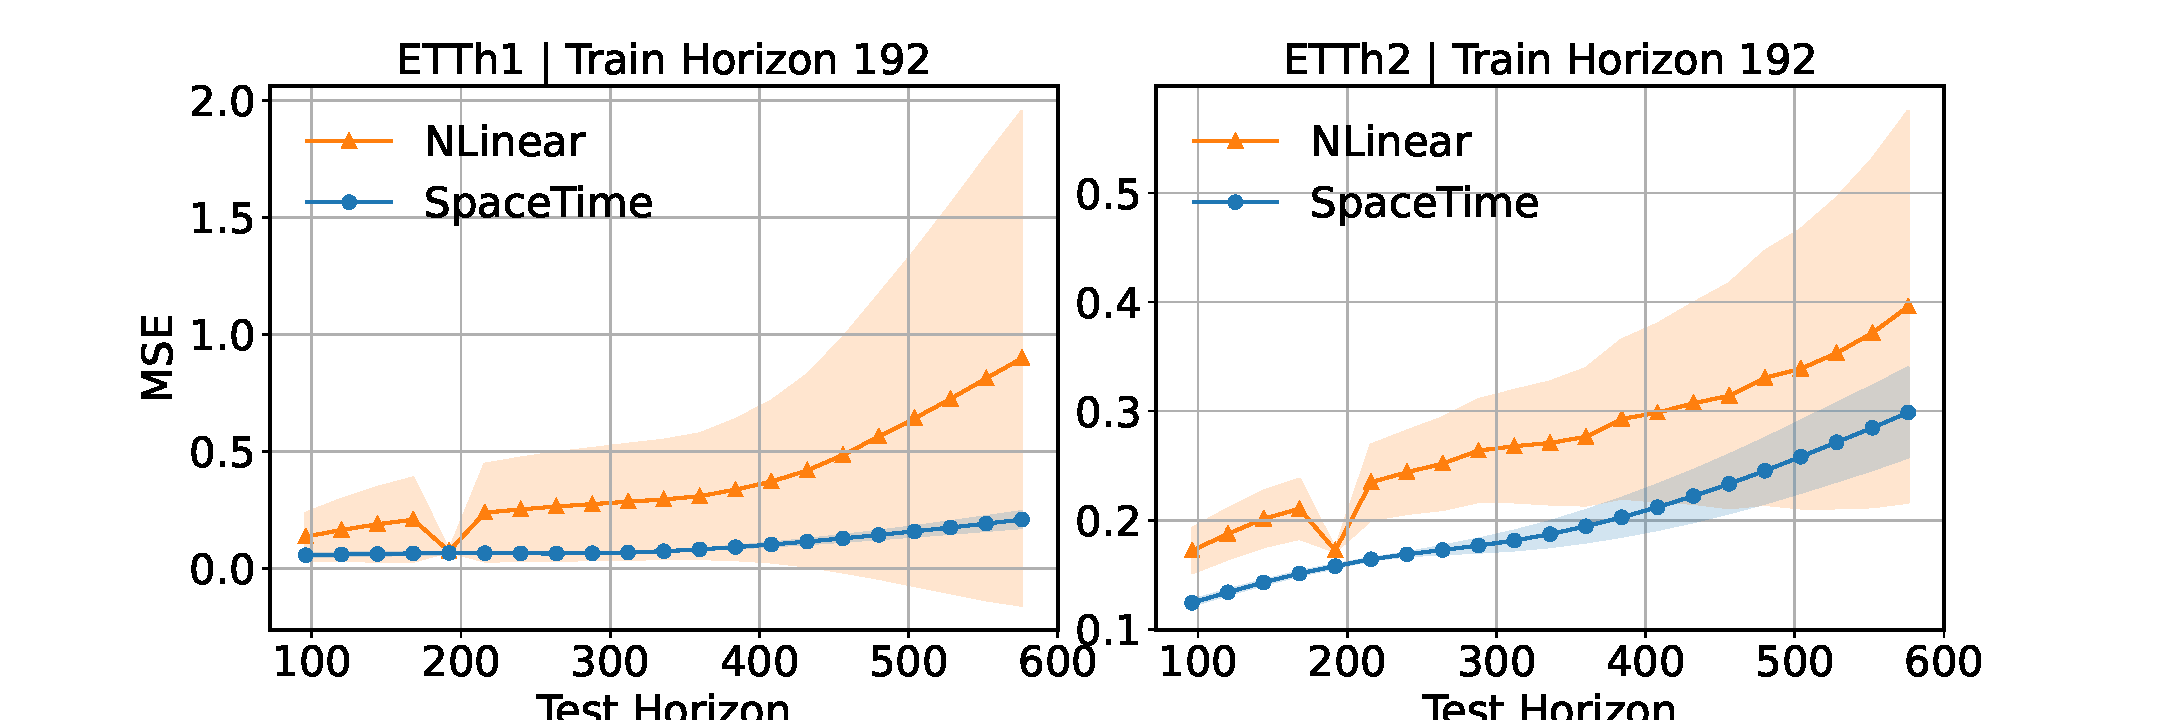
\includegraphics[width=1.125\linewidth]{_ICLR2023_paper/figures/ett_forecast_transfer.pdf}
  \caption{ \textbf{Forecasting transfer}. Mean MSE ($\pm 1$ standard deviation). \ourmethod{} 
%   trained to predict 192 time-steps 
  transfers more accurately and consistently to horizons not used for training versus NLinear~\cite{zeng2022transformers}.}
  \label{fig:transfer_forecast_etth} 
\end{minipage}
% \vspace{-0.65cm}
% \vspace{-0.55cm}
\end{figure}

\subsubsection{Long Horizon Forecasting} 
\label{sec:empirical_horizons}
To next study \ourmethod{}'s improved long horizon forecasting capabilities, we consider two additional long horizon tasks. 
%
First, we test on much longer horizons than prior settings (\cf{} Table~\ref{tab:informer-s-long}). Second, we test a new forecasting ability: how well methods trained to forecast one horizon transfer to longer horizons at test-time.  
%
For both, we use the popular Informer ETTh datasets. We compare \ourmethod{} with NLinear---the prior state-of-the-art on longer-horizon ETTh datasets---an FCN that learns a dense linear mapping between every lag input and horizon output~\citep{zeng2022transformers}.

We find \ourmethod{} outperforms NLinear on both long horizon tasks. On training to predict long horizons, \ourmethod{} consistently obtains lower MSE than NLinear on all settings (Table~\ref{tab:long_horizon_etth}). 
On transferring to new horizons, \ourmethod{} models trained to forecast 192 time-step horizons transfer more accurately and consistently to forecasting longer horizons up to 576 time-steps (Fig.~\ref{fig:transfer_forecast_etth}).
This suggests \ourmethod{} more convincingly learns the time series process; rather than only fitting to the specified horizon, the same model can generalize to new horizons.


% and further confirms that autoregressive methods can outperform direct multi-step approaches. 
%
% By more accurately generalizing to horizons not explicitly trained on, \ourmethod{}
%
% We find this result particularly interesting, as while all supervised time series methods are trained with some target horizon, models should perform well by learning the underlying time series process, and not just fitting to the specific training horizon. While DLinear obtains comparable results when the training and test horizons are equal (\cf{} 192 time-steps in Fig.~\ref{fig:transfer_forecast_etth}), it transfers worse to both shorter and longer new horizons, suggesting that \ourmethod{}'s forecasting mechanism captures the underlying time series processes more accurately.
%
%These results suggest \ourmethod{}'s forecasting mechanism allows it to not only more accurately forecast long horizons on real data, but also better learn their underlying time series processes.


\begin{figure}[H]
\begin{minipage}[c]{0.45\textwidth}
\centering
\captionof{table}{ \textbf{Train wall-clock time}. Seconds per epoch when training on ETTh1 data.}\label{tab:wallclock_etth}
\resizebox{1\linewidth}{!}{
\tabcolsep=0.3cm
\begin{tabular}{@{}lcc@{}}
    \toprule
    Method & \# params & seconds/epoch   \\
    \midrule
    \ourmethod{}& 148k & 66  \\
    $\rightarrow$ No Algorithm~\ref{alg:output_filter_computation} & 148k & 132  \\
    \midrule
    S4 & 151k & 49  \\
    % \midrule
    Transformer & 155k & 240 \\
    % \midrule
    LSTM & 145k & 336 \\
    \bottomrule
    \end{tabular}%
}
\end{minipage}
\quad
\begin{minipage}[c]{0.45\textwidth}
\centering
 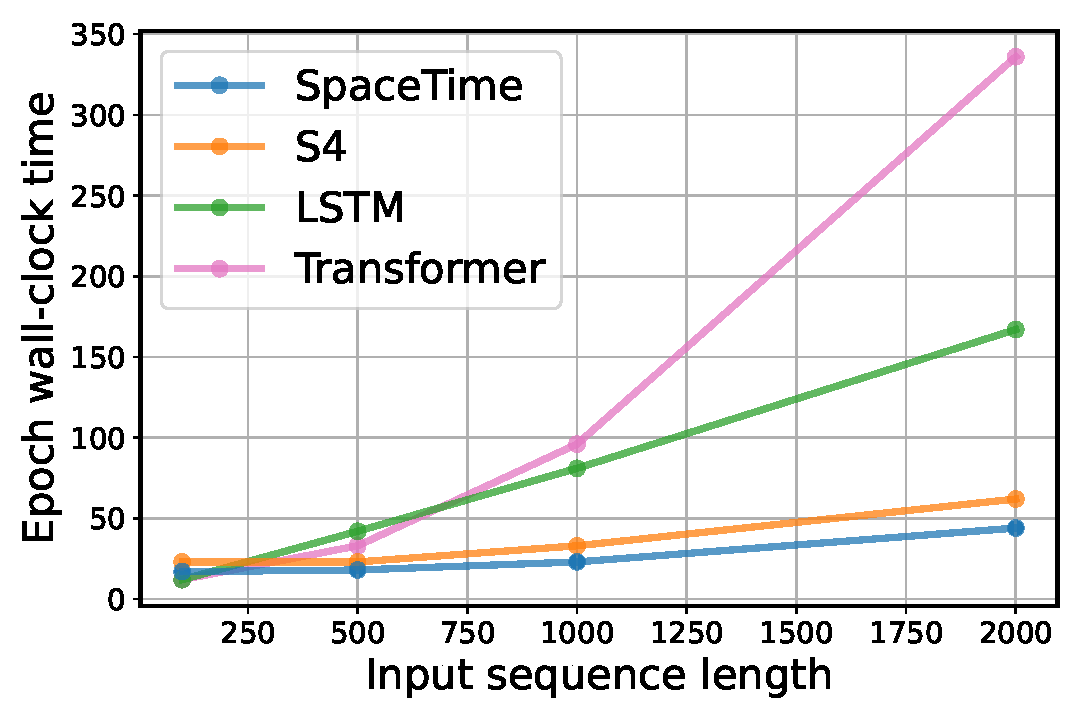
\includegraphics[width=1\textwidth]{_ICLR2023_paper/figures/speed_benchmark_square.pdf}
  \caption{ \textbf{Wall-clock time scaling}. Empirically, \ourmethod{} scales near-linearly with input sequence length.}
  \label{fig:wallclock_synth} 
\end{minipage}
\end{figure}


\subsubsection{Efficiency}
 \label{sec:empirical_efficiency}
To finally study if our companion matrix algorithm enables efficient training on long sequences, 
% To validate the advantage of \ourmethod's efficient training on long sequences, 
we conduct two speed benchmarks. We (1) compare the wall-clock time per training epoch of \ourmethod{} to standard sequence models, \eg{} LSTMs and Transformers, with similar pararemeter counts, and (2) empirically test our theory in Sec.~\ref{sec:efficient_algorithm}, which suggests \ourmethod{} trains near-linearly with sequence length and state dimension. For (1), we use ETTh1 data with lag and horizon 720 time-steps long. For (2), we use synthetic data, scaling sequences from 100$-$2000 time-steps long. 

%  \begin{wrapfigure}{r}{0.3\textwidth}
% \vspace{-2cm}
%   \begin{center}
%     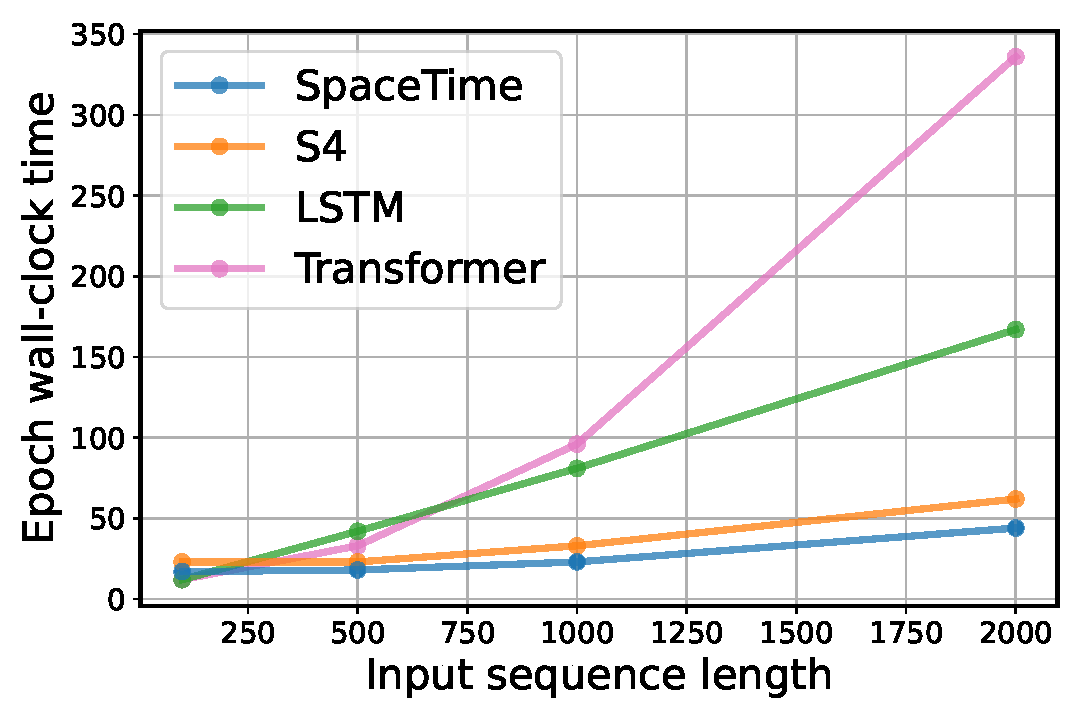
\includegraphics[width=0.3\textwidth]{_ICLR2023_paper/figures/speed_benchmark_square.pdf}
%  \vspace{-0.25cm}
%   \end{center}
%   \caption{\small \textbf{Wall-clock scaling}. \ourmethod{} trains fastest and scales near-linearly in input length.}
%   \label{fig:wallclock_synth} 
%   \vspace{-0.5cm}
% \end{wrapfigure}




% We compare wallclock time on a real dataset (ETTh1 forecasting with context and horizon length $720$) and on synthetic random data where we scale the input sequence length from $100$ to $2000$.

% We next empirically validate the efficient training capabilities of \ourmethod{}, where we expect the training time to scale (almost) linearly with input sequence length and state dimension, as theoretically shown in Section\ref{sec:efficient_algorithm} .

On (1) we find \ourmethod{} reduces clock time on ETTh1 by 73\% and 80\% compared to Transformers and LSTMs (Table \ref{tab:wallclock_etth}). Our efficient algorithm (Sec.~\ref{sec:efficient_algorithm}) is also important; it speeds up training by 2$\times$, and makes \ourmethod{}'s training time competitive with efficient models such as S4. On (2), we find \ourmethod{} also scales near-linearly with input sequence length, 
% and is significantly faster than Transformers and LSTMs, 
achieving 91\% faster training time versus similarly recurrent LSTMs (Fig.~\ref{fig:wallclock_synth}).




% \begin{figure}[h]
% \begin{minipage}[c]{0.35\textwidth}
% \vspace{-0.75cm}
% \centering
% \captionof{table}{\small \textbf{Train wall-clock time}. Seconds per epoch for ETTh1 forecasting.}\label{tab:wallclock_etth}
% \resizebox{1\linewidth}{!}{
% \tabcolsep=0.1cm
%   \begin{tabular}{@{}lcc@{}}
%     \toprule
%     Method & \# params & sec/epoch   \\
%     \midrule
%     \ourmethod{}& 148k & 66  \\
%     $\rightarrow$ No Algorithm~\ref{alg:output_filter_computation} & 148k & 132  \\
%     \midrule
%     S4 & 151k & 49  \\
%     % \midrule
%     Transformer & 155k & 240 \\
%     % \midrule
%     LSTM & 145k & 336 \\
%     \bottomrule
%     \end{tabular}%
% }
% \end{minipage}
% \quad
% \begin{minipage}[c]{0.35\textwidth}
% \vspace{-0.35cm}
% \centering
%  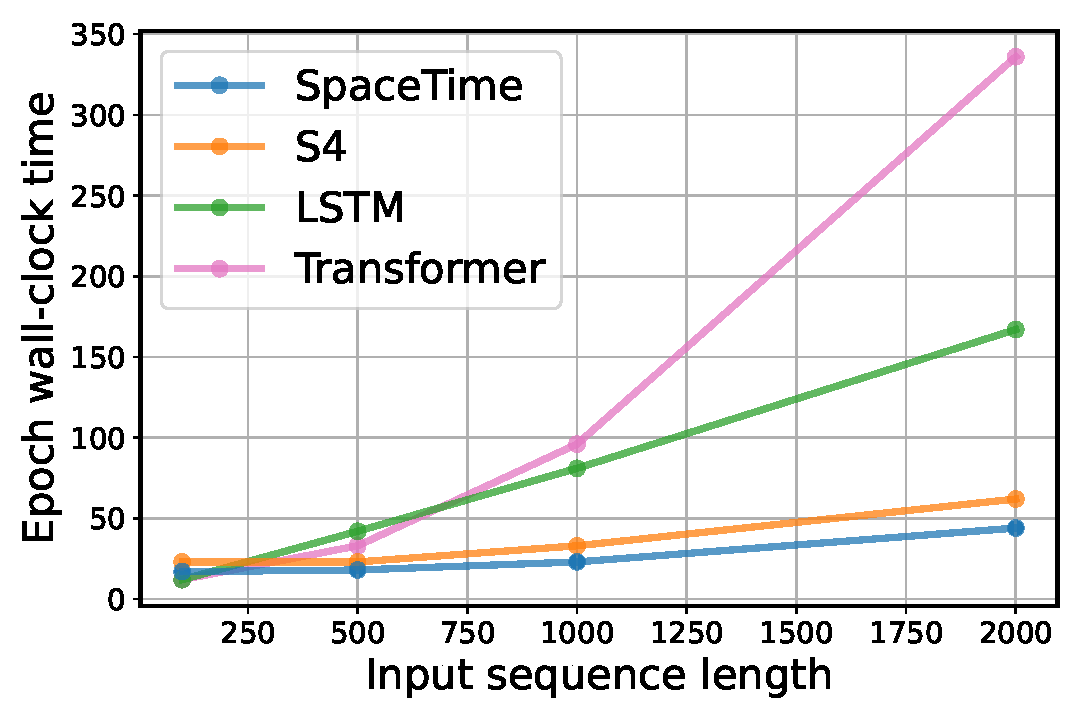
\includegraphics[width=0.9\textwidth]{_ICLR2023_paper/figures/speed_benchmark_square.pdf}
%  \vspace{-0.2cm}
%   \caption{\small \textbf{Wall-clock scaling}. Wall-clock time per epoch for sequence model training. \ourmethod{} trains fastest and scales near-linearly in input length.}
%   \label{fig:wallclock_synth} 
% \end{minipage}
% \vspace{-0.75cm}
% \end{figure}

%\subsection{Validate proposed \ourmethod{} components with ablations}

